% !TEX TS-program = pdflatex
\documentclass[10pt,twocolumn]{article} 

% required packages for Oxy Comps style
\usepackage{oxycomps} % the main oxycomps style file
\usepackage{times} % use Times as the default font
\usepackage[style=numeric,sorting=nyt]{biblatex} % format the bibliography nicely 

\usepackage{amsfonts} % provides many math symbols/fonts
\usepackage{listings} % provides the lstlisting environment
\usepackage{amssymb} % provides many math symbols/fonts
\usepackage{graphicx} % allows insertion of grpahics
\usepackage{hyperref} % creates links within the page and to URLs
\usepackage{url} % formats URLs properly
\usepackage{verbatim} % provides the comment environment
\usepackage{xpatch} % used to patch \textcite
\usepackage{algorithm,algpseudocode}

\graphicspath{ {../readme_images/} }

\bibliography{refs.bib}

% All from https://tex.stackexchange.com/questions/69728/indenting-lines-of-code-in-algorithm, allows for code indents
\newlength\myindent
\setlength\myindent{2em}

\newcommand\bindent{%
  \begingroup
  \setlength{\itemindent}{\myindent}
  \addtolength{\algorithmicindent}{\myindent}
}
\newcommand\eindent{\endgroup}
% Ends here


\DeclareNameAlias{default}{last-first}

\xpatchbibmacro{textcite}
  {\printnames{labelname}}
  {\printnames{labelname} (\printfield{year})}
  {}
  {}

\pdfinfo{
    /Title (Implementing and Evaluating K-Means Clustering)
    /Author (Christopher Linscott)
}

\title{Implementing and Evaluating K-Means Clustering}

\author{Christopher Linscott}
\affiliation{Occidental College}
\email{clinscott@oxy.edu}

\begin{document}

\maketitle

% Refer to rubric: https://docs.google.com/document/d/1oiXngqxh30ADXVPfOEnNuBNX1DGFmmExI6DoGZNdrs0/edit

\section {Abstract}

% The following tutorial report dives into two clustering algorithms, Fuzzy C Means and K Means, and implements them from scratch in Python with the help of online tutorials. After, sklearn's K-Means algorithm was tested on blobs of datapoints, pixels of an image, and batches of images to visualize and understand (through implementation) how the algorithms worked. Finally, the K-Means algorithm is evaluated on an iris-flower image dataset using a confusion matrix, elbow method, classification report, and Davies-Bouldin Score as different metrics to determine the strength of the algorithm. Finally, these metrics are reported and discussed to understand how the evaluation metrics worked and where the K-Means is strong and weak. While the K-Means algorithm was found to perform well in clustering these images, there are many caveats to this result including lack of other comparisons and frictions in reproducibility due to the lack of identified classes in clustering needed for classification metrics.

The following tutorial report dives into the K Means clustering algorithm, implementing it from scratch in Python with the help of online tutorials. After, sklearn's K-Means algorithm was tested on blobs of datapoints, pixels of an image, and batches of images to visualize and understand (through implementation) how the algorithms worked. Finally, the K-Means algorithm is evaluated on an iris-flower image dataset using a confusion matrix, elbow method, classification report, and Davies-Bouldin Score as different metrics to determine the strength of the algorithm in clustering batches of images. These metrics are reported and discussed to understand and conclude on K-Means's strengths and weaknesses. While the K-Means algorithm was found to cluster images proficiently overall, K-Means struggled with images of high similarity, but slight difference (like the iris virginica and iris versicolor flower).

\section {Methods}

\subsection {Approach/Framework}

The general approach to grouping images or any form of data point is the idea of clustering, where the main goal is to “...[segment] a population into subgroups where members are more similar to each other… based on certain observed features” \cite{C3Clustering}. Being able to separate images means being able to separate them apart based on their differences in objects, shapes, or environment. The main goal is not to recognize the objects, but to recognize meaningful differences or similarities between two images based on their visual similarity. Therefore, unlike with clustering simple blobs or batches of data points, to cluster images requires “cluster[ing] pixels into different image regions, which are regions corresponding to individual objects, surfaces or natural parts of the objects” \cite{Roy2014}. As this is an unsupervised version of machine learning (allowing for mainly testing), there is no response “class”, so a human needs to associate meaning with each cluster it generates.

With the help of tutorials \cite{Khushijain2021, Jordan2018, Aktas2021}, I implemented the K-Means algorithms from scratch, utilized K-Means from the sklearn library on three different examples: batches of data points, the pixels of a given image, and batches of images. The sklearn library was utilized, as opposed to the original implementation which could only cluster on datapoints of 1 or 2 dimensions which is too few for a batch of images or the pixels of an image. Before clustering each of these data formats, I preprocessed them using functions such as OpenCV’s image read function to load images, creating arrays of data points of 5 dimensions to represent its position and the values for each color channel (red, green, blue). To cluster only on the colors of the pixels, numpy’s reshape function was utilized to extract only the values from each color channel, creating three-dimensional data points. After performing sklearn’s K-Means algorithm on these data points, by utilizing the algorithm’s labels for each datapoint’s cluster, I combined each cluster’s data points into a single 2-D array, creating a 3-D array of \(k\) rows of 2-D arrays containing these data points; \(k\) represents the user-inputed number of clusters. The following arrays of data points were plotted using matplotlib, coloring pixels of the same cluster (i.e. in the same 2-D array) to show the results of the full clustering.

% The two clustering algorithms employed are Fuzzy C-Means and K-Means. With the help of tutorials \cite{Khushijain2021,TheAcademician2020, Jordan2018,Aktas2021}, I implemented both algorithms from scratch, utilized K-Means from the sklearn library on three different examples: batches of data points, the pixels of a given image, and batches of images. Before clustering each of these data formats, I preprocessed them using functions such as OpenCV’s image read function to load images, creating arrays of data points of 5 dimensions to represent its position and the values for each color channel (red, green, blue). To cluster only on the colors of the pixels, numpy’s reshape function was utilized to extract only the values from each color channel, creating three-dimensional data points. After performing sklearn’s K-Means algorithm on these data points, by utilizing the algorithm’s labels for each datapoint’s cluster, I combined each cluster’s data points into a single 2-D array, creating a 3-D array of \(k\) rows of 2-D arrays containing these data points; \(k\) represents the user-inputed number of clusters. The following arrays of data points were plotted using matplotlib, coloring pixels of the same cluster (i.e. in the same 2-D array) to show the results of the full clustering. 

For clustering batches of images, by utilizing the digits and iris datasets, the data points were extracted as a property (being accessed through .data) after executing a function to load the data. After clustering, we had the K-Means cluster and predict what images were in each cluster. Using the matplotlib library, we could plot these clusters and the corresponding images in sequence to visualize/show what K-means predicted. With clustering the images from the digits dataset (in particular), the digits beforehand were preprocessed to have their pixel values inverted by subtracting the pixel value from 255. These are primarily gray-scaled images, with the majority of the pixels being black or dark gray. By inverting the pixel values, the clustering algorithm will have an easier time clustering as it needs to only cluster on the dark pixels primarily.

\subsection {Datasets}

The datasets used by both my algorithms and my evaluation came from two of the seven toy datasets included in the sklearn library \cite{skLearn2020}, the iris data set and the digits data set. Not only do these datasets contain a large number of instances and classes, but unlike other datasets, getting the ground truth is much simpler and make evaluation much easier (compared to something like the BSDS500). The iris data set includes 150 different instances of iris flowers, with three different classes of iris flowers of 50 instances each; each class here refers to a type of iris plant. The digits data set includes 1797 instances of digits, or 8-bit images; the colors or pixel values range from 0 to 16. The digits data set has 10 different classes, each referring to a digit from 0 to 9. 


\subsection {Algorithms}

\subsubsection {K-Means}

A very well-known, partition-type clustering algorithm is K-Means. Partition-based clustering refers to a harder (meaning more strict) form of partitioning where every data point can only be in one cluster. The main goal of this algorithm is to create partitions of data points, by creating points of relevance called clusters, which minimize the distance from any given data point to any given cluster. The distance metric utilized by K-Means is Euclidean distance where the distance from a data point \(x_i\) to a cluster \(x_j \) with d dimensions can be calculated by:
\(D_{i, j} = \sum_{l=1}^d \sqrt{|x_{il}^2 - x_{jl}^2|} \). In my own implementation (for learning, understanding, and documentation), I utilized Euclidean distance for only 2 dimensions via: \(D_{i, j} = \sqrt{{|x_{j} - x_{i}|^2} + {|y_{j} - y_{i}|^2}} \). \\ In combination with my own implementation, I utilized Lloyd’s algorithm to compute and converge on centers of clusters, which is the same as for the library utilized in the tutorial, sklearn \cite{skLearnKMeans2020}.

% \subsubsection {Fuzzy C Means}

% The soft (fuzzy) counterpart to the K-Means algorithm is the Fuzzy C-Means (FCM) algorithm. The FCM algorithm is “softer” or “fuzzier” as unlike K-Means, it allows for a data point to coexist in several different clusters with different values of membership (i.e. how much it relates to that given cluster). In comparison to the K-Means, the FCM algorithm is more popular for image segmentation because it’s more computational efficient (O(n) versus O(knt) \cite{Mittal2021}, applicable to multichannel data (i.e. colored images), and has the ability to model uncertainty in the data \cite{Roy2014}. In the context of the high number of pixels being grouped upon, as well as the channels of color which apply to colored images, it’s clear that an algorithm like Fuzzy C Means is a very good option for image segmentation.

% Fuzzy C-Means, in a very similar fashion to K-Means, will utilize a Euclidean distance metric. However, FCM utilizes membership values of the data points, where every data point has a set of k membership values adding up to 1, with k being the number of clusters. These membership values will be randomly initialized for each data point, and tweaked depending on the distance metric from a data point to a cluster. The centers of the cluster will now be tweaked based on the mean of the data points as well as their membership values. In other words, the centroid’s data point will be most affected by data points which have a membership value high for that cluster. Mathematically, this is all represented by first calculating the centroid positions by computing \[ C_j = \frac{ \sum_{i}^{n} (m_{ij})^f * dp_i  }{  \sum_{i}^{n} (m_{ij})^f  }\] with \(n\) data points \(dp\), a cluster \(j\) and a given membership value of a data point \(i\) for a cluster \(j\) \(m_{ij}\). The new f value represents the fuzzifier, or what will convert a hard output into a soft output (i.e. less hard clustering); a value of 1 equates to K-Means, whereas infinity equates to all values being equally in the same cluster. After computing the new centroid values, the data point’s membership values will be equal to the euclidean distance from a data point i to cluster j, divided by the total euclidean distance to all clusters from the same data point. This is calculated as follows: \[m_{ij} = \frac{1}{\sum_{z=1}^{k} (\frac{|dp_i - c_j|}{|dp_i - c_z|})^{\frac{1}{f-1}}} \]

% \subsubsection {Pseudocode}

% \begin{algorithm}
%   \caption{ K-Means: Lloyd's Algorithm }
%   \textbf{Input:} \\
%   \textit{k}: number of clusters \\
%   \textit{data points} : array of data points of size n * d \\
%   \indent ($n$ = number of data points, $d$ = number of dimensions per data point) \\
%   \textbf{Output:} \\
%   \textit{centroids}: positions of the centroids (arr of size k * d) \\
%   \textit{clusters}: nearest cluster for each data point (arr of size n) \\
%   \begin{algorithmic}[1]
%     \State Initialize all data points to be in one cluster (to modify later), i.e. $ clusters = [0, ..., 0]$
%     \State Select k random data points' positions to be the initial positions for the centroids

%     \While {centroid positions change}
%      \For {$i \rightarrow n$ data points}
%       \For {$j \rightarrow k$ clusters} 
%       \State Calculate distance from data point i to cluster j
%       \State Keep track of the closest cluster
%       \EndFor 
%       \State Store new closest cluster $l$ for each data point i ($clusters[i] = l$)
%       \EndFor
%       \State $$C_j = \sum_{x_i \in C_j} \frac{x_i}{n}$$
%       New centroid position is the avg. of all its subsequent data point positions (refer to equation above)
%       $$ centroids[j] = C_j$$
%     \EndWhile \\
%   \textbf{Returns} \textit{centroids, clusters}
%   \end{algorithmic}
% \end{algorithm}

% \begin{algorithm}
%   \caption{ Fuzzy C-Means }
%   \textbf{Input:} \\
%   \textit{k}: number of clusters \\
%   \textit{data points} : array of data points of size n * d \\
%   \indent ($n$ = number of data points, $d$ = number of dimensions per data point) \\
%   \textit{f} : softness of clustering $(2 < f < \infty)$\\
%   \textbf{Output:} \\
%   \textit{centroids}: positions of the centroids (arr of size k * d) \\
%   \textit{clusters}: nearest cluster for each data point (arr of size n)
%   \begin{algorithmic}[1]
%     \State Initialize all membership values for each data point to be k random values which add to 1. 
%     \State Set initial centroid positions to be at $[0, ..., 0]$

%     \While {centroid positions change}
%      \For {$i \rightarrow k$ clusters}
%       \For {$j \rightarrow n$ clusters} 
%       \State Calculate new centroid positions $(C_j)$ using membership values
%       \EndFor 
%       \EndFor \\
%     \For {$i \rightarrow n$ data points}
%       \For {$j \rightarrow k$ clusters} 
%         \State Recalculate the membership values $m_{ij}$ with the new centroid positions
%       \EndFor
%       \EndFor
%     \EndWhile \\

%     Initialize clusters array with the cluster corresponding to each data point's highest membership value \\
%   \textbf{Returns} \textit{centroids, clusters}
%   \end{algorithmic}
% \end{algorithm}

\section {Evaluation}

Evaluation of the K-Means algorithm was performed using the iris and digits datasets proposed in the Datasets section of this paper. A confusion matrix, elbow method, classification report, and Davies-Bouldin Score were all utilized to generate different metrics of accuracy of the clustering algorithms; all of this metrics came as well from the sk-learn library. By comparing the predictions versus the truth, we can determine the strength of the clusters by determining if objects (flowers) of the same class are grouped together (i.e. using classification evaluation methods). As we cluster upon images, these metrics can show the strength of the clustering algorithm upon images of related visual characteristics, and whether they can separate highly similar, but different images.

The first proposed method was a confusion matrix, where given the ground truth and the predictions, it will plot the numbers of correct and incorrect predictions in a matrix, with the correct predictions along the main diagonal (top left corner to bottom right corner) and the incorrect predictions on either side of the main diagonal; false negatives were on the top right side and false positive on the bottom left side. Given the class names (i.e. what digits or flowers), the Confusion Matrix can specifically tell which classes the algorithm struggled to cluster. The Confusion Matrix can help us visualize how accurate the clusters are (besides giving us a plain number), by showing the number of relevant objects clustered with each other. 

The second proposed method was Davie Boulden's Score, which can assess the strength of a clustering algorithm without knowing the ground truth. The score is defined as the "average similarity measure of each cluster with its most similar cluster, where similarity is the ratio of within-cluster distances to between-cluster distances" \cite{skLearn2020}. The minimum and best possible score is zero, with lower values indicating better clustering. Not only can this tell us the strength without the dataset, but it can be compared amongst other algorithms easily as a baseline.

The third proposed method was the Classification Report, which when given the ground truth and prediction, can quickly calculate and give information about accuracy, precision, recall, and f1-score of the clustering algorithm by computing various ratios/formulas as shown where \(TP\) means the number of "true" predictions where the model predicts the correct class, \(TN\) means the number of true "false" predictions where the model predicts the image is not a given class, \(FN\) refers to the number of false negatives where the model falsely predicts an image is not a given class (but it truly is), and a \(FP\) refers to the number of false positives where the model says incorrectly that an image is of a certain class when it's in truth another one. The classification report can give us a further idea of what relevant images were clustered properly and calculate the following metrics of precision \(P\), recall \(R\), accuracy \(A\), and F1-score \(F1\). These metrics can help us determine if the clustered items are relevant to each other, if relevant items are retrieved, the overall accuracy, and the f1-score is a combined measurement of both the precision and recall (together).

\[P = \frac{TP}{TP + FP}\]
\[R = \frac{TP}{TP + FN}\]

\[A = \frac{TP + TN}{TP + TN + FP + FN}\]
\[F1 = \frac{2 * P * R}{P + R}\]

The final method, the "Elbow" Method evaluates the best number of clusters for clustering the given data; this is very useful for clustering algorithms such as FCM or K-Means where the number of clusters must be given. The main idea behind the Elbow Method is plotting the WCSS (Within Cluster Sum Square), which is the sum of the squared distance between each point and the centroid in the cluster; the squared distance can be calculated by square rooting the Euclidean distance differences for every data point in the cluster j:

\[\sqrt{\sum_{x_i \in c_j}(x_{i} - c_{j})^2}\]

As you plot more clusters, WCSS will decrease at a slower rate, and have diminishing returns. Once the graph begins to have a second bend, much like an elbow, where the elbow is formed tells you the best number of clusters. The Elbow Method, from an evaluation standpoint, can also tell us if the rough number of classes in the data can be determined; it tell us how well the clustering algorithm sees the differences. If the clustering algorithm sees the images as the same, the elbow will form at a low number (which is not what we want).

\subsection{Results}
After performing the following evaluation methods on the K-Means algorithm with the Iris Dataset, we obtained the following results:

\begin{figure}[h]
  \centering
  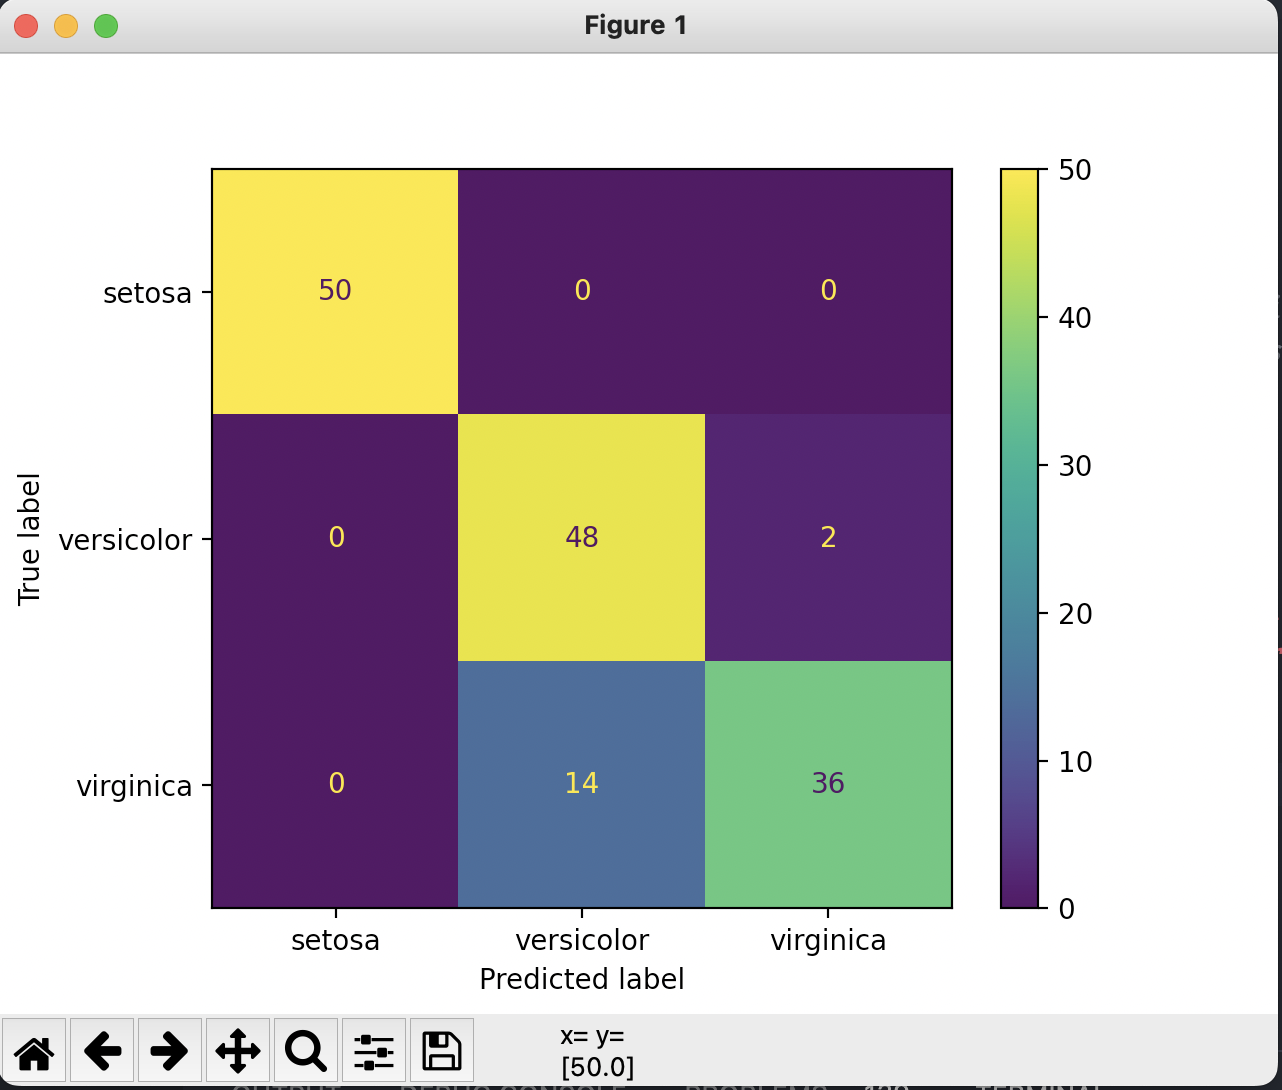
\includegraphics[scale=0.3]{confusion_matrix.png}
  \vspace{20px}
  \caption{The Confusion Matrix generated after clustering upon 150 flowers of three different possible classes, with the K-Means algorithm.}
  \label{confusion_matrix}
\end{figure}

\begin{figure}[H]
  \centering
  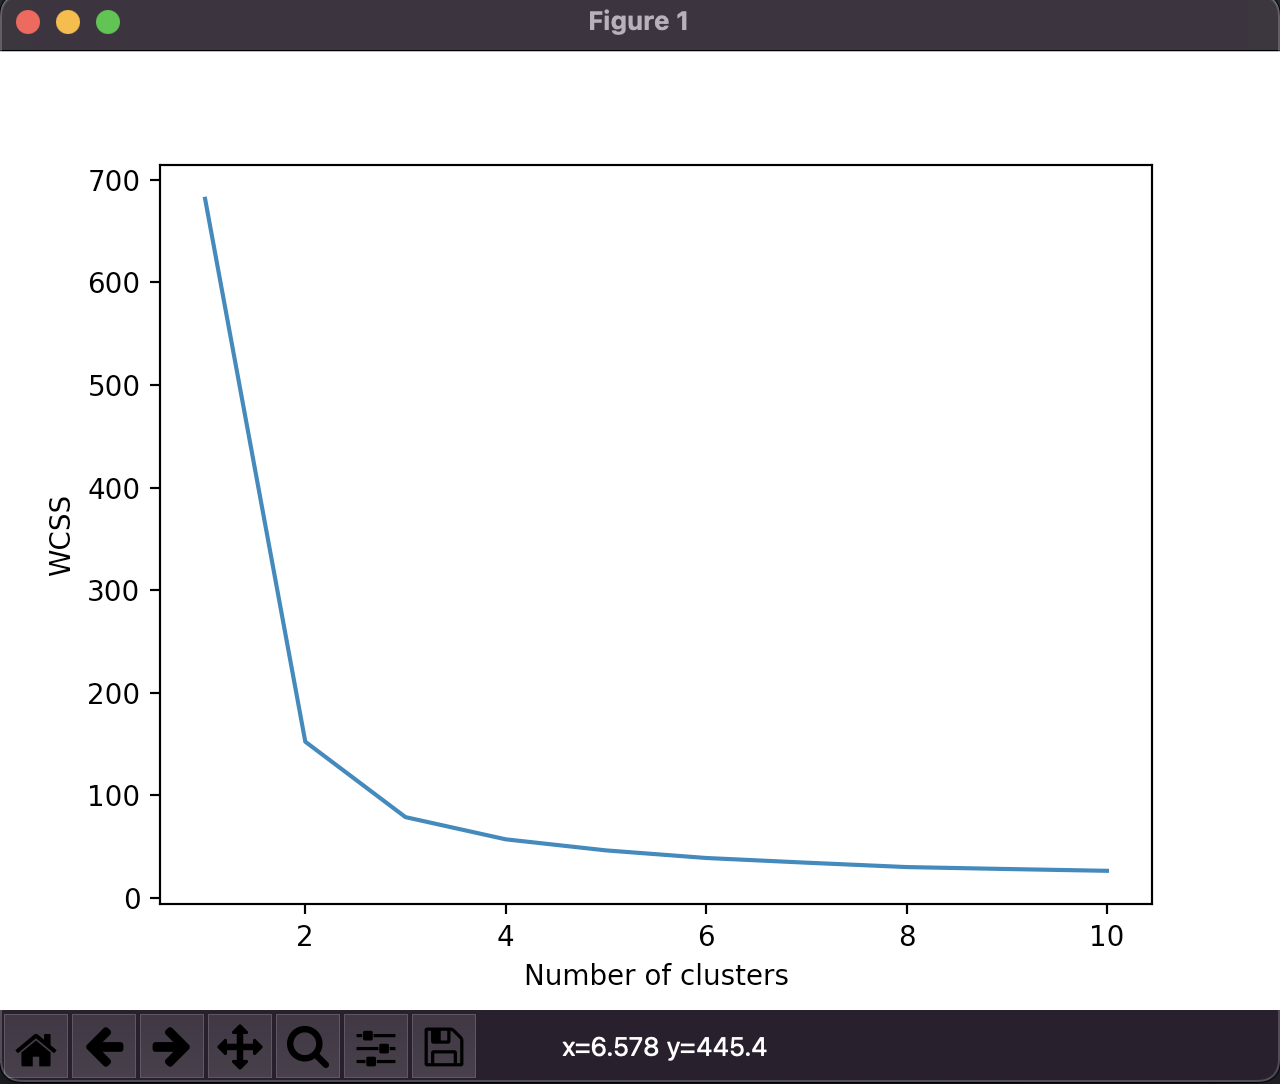
\includegraphics[scale=0.3]{iris_elbow.png}
  \vspace{20px}
  \caption{The WCSS versus Number Of Clusters (for the Elbow Method). The best number of clusters should be 3.}
  \label{iris_elbow}
\end{figure}

\begin{figure}[h!]
  \centering
  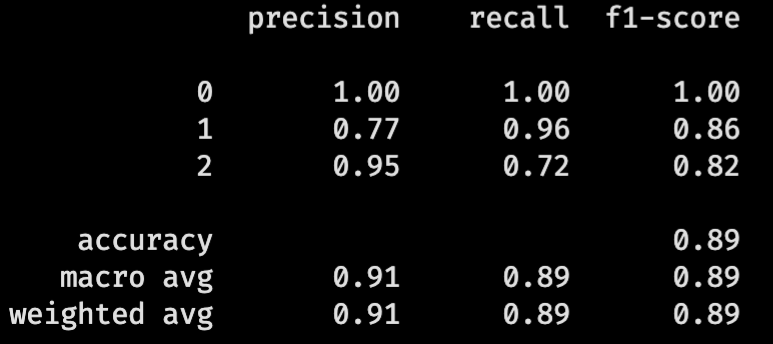
\includegraphics[scale=0.3]{class_report_iris.png}
  \vspace{20px}
  \caption{The classification report of the clustering by K-Means on the Iris Dataset. Each class was evaluated on its precision, recall, and f1-score. The overall accuracy is summed up.}
  \label{class_report_iris}
\end{figure}

As well as, the generated Davie-Boulden's Score was 0.66, which is very strong considering its proximity to 0.

\section {Discussion}

% Dicussion = what results we got and why, the caveats of our results

% Software Documentation = instructions for installing your code
% A basic overview of how your code works

The results we got above are proficient and expected, but have minor issues. As we clustered upon the three different possible classes, the "elbow" formed around k = 3 clusters; this is the appropriate and expected number of clusters to work best roughly (since there are 3 classes of flowers). Additionally, the low Davie-Boulden's score shows that the clusters are more tightly knit, and that the clustering algorithm was able to differentiate between the images of the flower well. The several metrics shown above showcase the ability for the clustering algorithm to group different images apart, but also the weaknesses in grouping highly similar, but slightly different images. The classification report, in combination with our confusion matrix, show the different scores across the different classes. As the first class (setosa) is different slightly in color and shape, the clustering algorithm clustered them all correctly (making the scores all 1s). 

However, it's clear that due to the close similarities between the virginica and versicolor plants, that the clustering algorithm had a much harder time clustering them as 16 plants between the two classes were not clustered correctly. To note, the precision of the algorithm was higher than the recall, showing its ability to cluster images well, but a weaker ability to cluster together relevant images. While the overall accuracy of the clustering algorithm is high, it's likely to decrease as the number of "similar, but different" images increases due to a lower recall. In the context of clustering images apart (for relevance), the K-Means clustering algorithm alone is not bad, but not good enough.

% the scores will all be ones, as the true positives and true negative will be equal to the total number of TP, TN, FN, FP since the false positives and false negatives are effectively zero. However, for the second and third classes, the precision and recall are opposite, as the number of false positives (14) for class 1 (which lowers the precision) corresponds to the number of false negatives for class 2 (which lowers the recall). As well as, the number of false negatives for class 1 (2) corresponds to the number of true positive for class 2. Therefore, the values of precision and recall will be similar, but opposite for these two classes (lowering their f1 score). Overall, the number of false positives and negatives (16) is relatively low in comparison to the entire 150 total instances, making the accuracy relatively high (0.9) as expected.

Not to mention, it doesn't show any comparisons to other clustering algorithms such as FCM or DBSCAN for example. The evaluations, while justified classification methods, all came from sk-learn library, and there is little diversity of evaluation overall. For the ease-of-use, these methods were utilized as they were already apart of the sklearn library (along with the dataset and algorithm), however other clustering evaluation methods (such as those deeper than David-Boulden's score) and even other classification methods could be utilized to test and evaluate the K-Means algorithm further.

% The algorithm evaluated came from the sk-learn library as opposed to my own implementation, as it can cluster data points of higher dimensions ($> 2$). Therefore, this doesn't evaluate the validity of my original implementations entirely (even if they're modeled similar to sklearn's algorithm). 

As a side note, these results are hard to reproduce, not because the clustering algorithm is incompetent, but due to the fact that clusters have no corresponding class to them. Therefore, the matching of "clusters" and classes is entirely random, and to reproduce these results takes a few reruns of the clustering algorithm and evaluation functions. Not only does this affect the results of the Classification Report, but this affects the Confusion Matrix produced, as the mismatch of class appears as False Positives and Negatives. While there is a clear reproducibility issue in this code, the methods are still viable; to reiterate, evaluating the clusters based on their accuracy (even via comparing classes) works as grouping images of similar visual context should group images of the same class together.



% To go further, while the classification report calculates the individual scores of precision, recall, and f1-score for classes, there is no overall score for all of them together. 


\printbibliography
 
\end{document}
